% ============================================
% BAB 4 - ANALISIS DAN PERANCANGAN SISTEM
% SISRI-BPI (Sistem Informasi Skripsi)
% Universitas Trunojoyo Madura
% ============================================

\chapter{ANALISIS DAN PERANCANGAN SISTEM}

\section{Analisis Sistem}

\subsection{Analisis Sistem yang Berjalan}
Sistem pengelolaan skripsi yang saat ini berjalan di Program Studi Teknik Informatika Fakultas Teknik Universitas Trunojoyo Madura masih menggunakan metode konvensional dengan beberapa permasalahan sebagai berikut:

\begin{enumerate}
    \item Pengajuan topik skripsi dilakukan secara manual melalui formulir fisik
    \item Proses persetujuan pembimbing membutuhkan waktu yang lama karena harus bertemu langsung
    \item Penjadwalan sidang dilakukan secara manual oleh koordinator
    \item Dokumentasi bimbingan tidak terstruktur dengan baik
    \item Tidak ada sistem notifikasi otomatis untuk mahasiswa dan dosen
\end{enumerate}

\subsection{Analisis Kebutuhan Sistem}

\subsubsection{Kebutuhan Fungsional}
Berdasarkan analisis permasalahan, sistem yang akan dibangun harus memenuhi kebutuhan fungsional sebagai berikut:

\begin{table}[H]
\centering
\caption{Kebutuhan Fungsional Sistem}
\label{tab:kebutuhan-fungsional}
\begin{tabular}{|c|l|p{8cm}|}
\hline
\textbf{No} & \textbf{Kode} & \textbf{Deskripsi} \\
\hline
1 & KF-01 & Sistem dapat mengelola data pengguna (admin, mahasiswa, dosen, koordinator) \\
\hline
2 & KF-02 & Sistem dapat mengelola pengajuan topik skripsi oleh mahasiswa \\
\hline
3 & KF-03 & Sistem dapat mengelola usulan dan persetujuan pembimbing \\
\hline
4 & KF-04 & Sistem dapat mencatat dan mengelola proses bimbingan \\
\hline
5 & KF-05 & Sistem dapat mengelola pendaftaran seminar proposal dan sidang skripsi \\
\hline
6 & KF-06 & Sistem dapat melakukan penjadwalan sidang secara otomatis \\
\hline
7 & KF-07 & Sistem dapat mengelola penilaian sidang \\
\hline
8 & KF-08 & Sistem dapat mengelola revisi pasca sidang \\
\hline
9 & KF-09 & Sistem dapat menghasilkan laporan dan statistik \\
\hline
\end{tabular}
\end{table}

\subsubsection{Kebutuhan Non-Fungsional}
\begin{table}[H]
\centering
\caption{Kebutuhan Non-Fungsional Sistem}
\label{tab:kebutuhan-non-fungsional}
\begin{tabular}{|c|l|p{8cm}|}
\hline
\textbf{No} & \textbf{Aspek} & \textbf{Deskripsi} \\
\hline
1 & Keamanan & Sistem menggunakan autentikasi berbasis session dan role-based access control \\
\hline
2 & Performa & Sistem dapat menangani minimal 100 pengguna secara bersamaan \\
\hline
3 & Usability & Antarmuka sistem mudah digunakan dan responsif \\
\hline
4 & Reliability & Sistem memiliki uptime minimal 99\% \\
\hline
5 & Scalability & Sistem dapat dikembangkan untuk menambah fitur baru \\
\hline
\end{tabular}
\end{table}

\subsection{Analisis Pengguna}
Sistem SISRI-BPI memiliki empat jenis pengguna dengan hak akses yang berbeda:

\begin{table}[H]
\centering
\caption{Analisis Pengguna Sistem}
\label{tab:analisis-pengguna}
\begin{tabular}{|c|l|p{9cm}|}
\hline
\textbf{No} & \textbf{Pengguna} & \textbf{Hak Akses} \\
\hline
1 & Admin & Mengelola seluruh data master, pengguna, dan konfigurasi sistem \\
\hline
2 & Mahasiswa & Mengajukan topik, melakukan bimbingan, mendaftar sidang, melihat nilai \\
\hline
3 & Dosen & Menyetujui pembimbingan, memberikan feedback bimbingan, menilai sidang \\
\hline
4 & Koordinator & Menyetujui topik, menjadwalkan sidang, mengelola periode akademik \\
\hline
\end{tabular}
\end{table}

% ============================================
\section{Perancangan Sistem}

\subsection{Arsitektur Sistem}
Sistem SISRI-BPI dibangun menggunakan arsitektur \textit{Model-View-Controller} (MVC) dengan framework Laravel. Arsitektur sistem ditunjukkan pada Gambar \ref{fig:arsitektur-sistem}.

\begin{figure}[H]
\centering
\begin{tikzpicture}[
    node distance=1.5cm,
    box/.style={rectangle, draw, rounded corners, minimum width=3cm, minimum height=1cm, align=center, fill=blue!10},
    arrow/.style={->, thick}
]
    % Client Layer
    \node[box, fill=green!20] (browser) {Web Browser\\(Client)};
    
    % Presentation Layer
    \node[box, below=of browser, fill=yellow!20] (view) {View Layer\\(Blade Templates)};
    
    % Application Layer
    \node[box, below=of view, fill=orange!20] (controller) {Controller Layer\\(HTTP Controllers)};
    
    % Business Logic Layer
    \node[box, below=of controller, fill=red!20] (model) {Model Layer\\(Eloquent Models)};
    
    % Data Layer
    \node[box, below=of model, fill=purple!20] (db) {Database\\(SQLite/MySQL)};
    
    % Arrows
    \draw[arrow, <->] (browser) -- (view);
    \draw[arrow, <->] (view) -- (controller);
    \draw[arrow, <->] (controller) -- (model);
    \draw[arrow, <->] (model) -- (db);
    
    % Labels
    \node[right=2cm of browser] {\textbf{Client Layer}};
    \node[right=2cm of view] {\textbf{Presentation Layer}};
    \node[right=2cm of controller] {\textbf{Application Layer}};
    \node[right=2cm of model] {\textbf{Business Logic Layer}};
    \node[right=2cm of db] {\textbf{Data Layer}};
    
\end{tikzpicture}
\caption{Arsitektur Sistem SISRI-BPI}
\label{fig:arsitektur-sistem}
\end{figure}

\subsection{Use Case Diagram}
Use case diagram menggambarkan interaksi antara aktor dengan sistem. Diagram use case sistem SISRI-BPI ditunjukkan pada Gambar \ref{fig:usecase}.

\begin{figure}[H]
\centering
\begin{tikzpicture}[
    actor/.style={},
    usecase/.style={ellipse, draw, minimum width=2.5cm, minimum height=1cm, align=center, font=\small},
    system/.style={rectangle, draw, dashed, minimum width=8cm, minimum height=12cm}
]
    % System boundary
    \node[system, label=above:{\textbf{SISRI-BPI}}] (system) at (5,0) {};
    
    % Actors
    \node at (-1, 4) (mahasiswa) {};
    \draw (-1, 4.5) circle (0.3);
    \draw (-1, 4.2) -- (-1, 3.5);
    \draw (-1, 4) -- (-0.5, 3.8);
    \draw (-1, 4) -- (-1.5, 3.8);
    \draw (-1, 3.5) -- (-0.5, 3);
    \draw (-1, 3.5) -- (-1.5, 3);
    \node at (-1, 2.7) {\small Mahasiswa};
    
    \node at (-1, -1) (dosen) {};
    \draw (-1, -0.5) circle (0.3);
    \draw (-1, -0.8) -- (-1, -1.5);
    \draw (-1, -1) -- (-0.5, -1.2);
    \draw (-1, -1) -- (-1.5, -1.2);
    \draw (-1, -1.5) -- (-0.5, -2);
    \draw (-1, -1.5) -- (-1.5, -2);
    \node at (-1, -2.3) {\small Dosen};
    
    \node at (11, 2) (koordinator) {};
    \draw (11, 2.5) circle (0.3);
    \draw (11, 2.2) -- (11, 1.5);
    \draw (11, 2) -- (11.5, 1.8);
    \draw (11, 2) -- (10.5, 1.8);
    \draw (11, 1.5) -- (11.5, 1);
    \draw (11, 1.5) -- (10.5, 1);
    \node at (11, 0.7) {\small Koordinator};
    
    \node at (11, -3) (admin) {};
    \draw (11, -2.5) circle (0.3);
    \draw (11, -2.8) -- (11, -3.5);
    \draw (11, -3) -- (11.5, -3.2);
    \draw (11, -3) -- (10.5, -3.2);
    \draw (11, -3.5) -- (11.5, -4);
    \draw (11, -3.5) -- (10.5, -4);
    \node at (11, -4.3) {\small Admin};
    
    % Use cases
    \node[usecase] (uc1) at (5, 5) {Login};
    \node[usecase] (uc2) at (3, 3.5) {Ajukan Topik};
    \node[usecase] (uc3) at (5, 2) {Bimbingan};
    \node[usecase] (uc4) at (3, 0.5) {Daftar Sidang};
    \node[usecase] (uc5) at (7, 3.5) {Setujui Topik};
    \node[usecase] (uc6) at (7, 1) {Jadwalkan\\Sidang};
    \node[usecase] (uc7) at (5, -1) {Nilai Sidang};
    \node[usecase] (uc8) at (3, -2.5) {Revisi};
    \node[usecase] (uc9) at (7, -2.5) {Kelola Data\\Master};
    \node[usecase] (uc10) at (5, -4.5) {Lihat Laporan};
    
    % Connections - Mahasiswa
    \draw (0, 4) -- (uc1);
    \draw (0, 4) -- (uc2);
    \draw (0, 4) -- (uc3);
    \draw (0, 4) -- (uc4);
    \draw (0, 3.5) -- (uc8);
    
    % Connections - Dosen
    \draw (0, -1) -- (uc1);
    \draw (0, -1) -- (uc3);
    \draw (0, -1) -- (uc7);
    \draw (0, -1) -- (uc8);
    
    % Connections - Koordinator
    \draw (10, 2) -- (uc1);
    \draw (10, 2) -- (uc5);
    \draw (10, 2) -- (uc6);
    \draw (10, 2) -- (uc10);
    
    % Connections - Admin
    \draw (10, -3) -- (uc1);
    \draw (10, -3) -- (uc9);
    \draw (10, -3) -- (uc10);
    
\end{tikzpicture}
\caption{Use Case Diagram SISRI-BPI}
\label{fig:usecase}
\end{figure}

\subsection{Activity Diagram}

\subsubsection{Activity Diagram Pengajuan Topik Skripsi}
\begin{figure}[H]
\centering
\begin{tikzpicture}[
    node distance=1cm,
    startstop/.style={circle, draw, fill=black, minimum size=0.5cm},
    process/.style={rectangle, draw, rounded corners, minimum width=3cm, minimum height=0.8cm, align=center, fill=blue!10},
    decision/.style={diamond, draw, aspect=2, minimum width=1.5cm, fill=yellow!20},
    arrow/.style={->, thick}
]
    % Start
    \node[startstop] (start) {};
    
    % Processes
    \node[process, below=of start] (p1) {Mahasiswa login};
    \node[process, below=of p1] (p2) {Pilih menu Topik Skripsi};
    \node[process, below=of p2] (p3) {Isi form pengajuan topik};
    \node[process, below=of p3] (p4) {Upload file proposal};
    \node[process, below=of p4] (p5) {Submit pengajuan};
    \node[decision, below=of p5] (d1) {Valid?};
    \node[process, below left=1cm and 1cm of d1] (p6) {Tampilkan error};
    \node[process, below right=1cm and 1cm of d1] (p7) {Simpan ke database};
    \node[process, below=2cm of d1] (p8) {Notifikasi ke Koordinator};
    
    % End
    \node[startstop, below=of p8] (end) {};
    \draw[fill=white] (end) circle (0.2cm);
    
    % Arrows
    \draw[arrow] (start) -- (p1);
    \draw[arrow] (p1) -- (p2);
    \draw[arrow] (p2) -- (p3);
    \draw[arrow] (p3) -- (p4);
    \draw[arrow] (p4) -- (p5);
    \draw[arrow] (p5) -- (d1);
    \draw[arrow] (d1) -- node[above] {Tidak} (p6);
    \draw[arrow] (d1) -- node[above] {Ya} (p7);
    \draw[arrow] (p6) |- (p3);
    \draw[arrow] (p7) |- (p8);
    \draw[arrow] (p8) -- (end);
    
\end{tikzpicture}
\caption{Activity Diagram Pengajuan Topik Skripsi}
\label{fig:activity-topik}
\end{figure}

\subsubsection{Activity Diagram Penjadwalan Sidang Otomatis}
\begin{figure}[H]
\centering
\begin{tikzpicture}[
    node distance=0.8cm,
    startstop/.style={circle, draw, fill=black, minimum size=0.5cm},
    process/.style={rectangle, draw, rounded corners, minimum width=3.5cm, minimum height=0.7cm, align=center, fill=blue!10, font=\small},
    decision/.style={diamond, draw, aspect=2, minimum width=1cm, fill=yellow!20, font=\small},
    arrow/.style={->, thick}
]
    % Start
    \node[startstop] (start) {};
    
    % Processes
    \node[process, below=of start] (p1) {Koordinator login};
    \node[process, below=of p1] (p2) {Pilih menu Jadwal Otomatis};
    \node[process, below=of p2] (p3) {Ambil pendaftaran\\status=menunggu};
    \node[process, below=of p3] (p4) {Ambil data ruangan\\dan slot waktu};
    \node[process, below=of p4] (p5) {Jalankan algoritma\\penjadwalan};
    \node[decision, below=of p5] (d1) {Konflik?};
    \node[process, right=2cm of d1] (p6) {Cari slot alternatif};
    \node[process, below=of d1] (p7) {Generate jadwal};
    \node[process, below=of p7] (p8) {Simpan pelaksanaan sidang};
    \node[process, below=of p8] (p9) {Kirim notifikasi};
    
    % End
    \node[startstop, below=of p9] (end) {};
    \draw[fill=white] (end) circle (0.2cm);
    
    % Arrows
    \draw[arrow] (start) -- (p1);
    \draw[arrow] (p1) -- (p2);
    \draw[arrow] (p2) -- (p3);
    \draw[arrow] (p3) -- (p4);
    \draw[arrow] (p4) -- (p5);
    \draw[arrow] (p5) -- (d1);
    \draw[arrow] (d1) -- node[above] {Ya} (p6);
    \draw[arrow] (p6) |- (p5);
    \draw[arrow] (d1) -- node[right] {Tidak} (p7);
    \draw[arrow] (p7) -- (p8);
    \draw[arrow] (p8) -- (p9);
    \draw[arrow] (p9) -- (end);
    
\end{tikzpicture}
\caption{Activity Diagram Penjadwalan Sidang Otomatis}
\label{fig:activity-jadwal}
\end{figure}

\subsection{Sequence Diagram}

\subsubsection{Sequence Diagram Proses Bimbingan}
\begin{figure}[H]
\centering
\begin{sequencediagram}
    \newthread{mhs}{Mahasiswa}
    \newinst[2]{ctrl}{Controller}
    \newinst[2]{model}{Model}
    \newinst[2]{db}{Database}
    
    \begin{call}{mhs}{submitBimbingan()}{ctrl}{response}
        \begin{call}{ctrl}{validate()}{ctrl}{valid}
        \end{call}
        \begin{call}{ctrl}{create()}{model}{bimbingan}
            \begin{call}{model}{insert()}{db}{success}
            \end{call}
        \end{call}
        \begin{call}{ctrl}{notify()}{model}{sent}
        \end{call}
    \end{call}
    
    \begin{sdblock}{alt}{Dosen Merespon}
        \begin{call}{mhs}{getStatus()}{ctrl}{status}
            \begin{call}{ctrl}{find()}{model}{data}
                \begin{call}{model}{select()}{db}{result}
                \end{call}
            \end{call}
        \end{call}
    \end{sdblock}
\end{sequencediagram}
\caption{Sequence Diagram Proses Bimbingan}
\label{fig:sequence-bimbingan}
\end{figure}

\subsection{Class Diagram}
Class diagram menggambarkan struktur kelas-kelas yang digunakan dalam sistem beserta relasinya.

\begin{figure}[H]
\centering
\begin{tikzpicture}[
    class/.style={rectangle, draw, minimum width=4cm, font=\small},
    classlabel/.style={rectangle, draw, fill=blue!20, minimum width=4cm, font=\small\bfseries}
]
    % User Class
    \node[classlabel] (user-label) at (0, 6) {User};
    \node[class, below=-0.02cm of user-label, text width=3.8cm, align=left] (user) {
        - id: int\\
        - name: string\\
        - email: string\\
        - password: string\\
        - role: enum\\
        + login()\\
        + logout()
    };
    
    % Mahasiswa Class
    \node[classlabel] (mhs-label) at (-5, 2) {Mahasiswa};
    \node[class, below=-0.02cm of mhs-label, text width=3.8cm, align=left] (mhs) {
        - nim: string\\
        - nama: string\\
        - angkatan: string\\
        - prodi\_id: int\\
        + ajukanTopik()\\
        + bimbingan()\\
        + daftarSidang()
    };
    
    % Dosen Class
    \node[classlabel] (dosen-label) at (5, 2) {Dosen};
    \node[class, below=-0.02cm of dosen-label, text width=3.8cm, align=left] (dosen) {
        - nip: string\\
        - nama: string\\
        - prodi\_id: int\\
        + setujuiPembimbing()\\
        + responBimbingan()\\
        + nilaiSidang()
    };
    
    % TopikSkripsi Class
    \node[classlabel] (topik-label) at (-5, -3) {TopikSkripsi};
    \node[class, below=-0.02cm of topik-label, text width=3.8cm, align=left] (topik) {
        - judul: string\\
        - status: enum\\
        - bidang\_minat\_id: int\\
        + submit()\\
        + approve()\\
        + reject()
    };
    
    % Bimbingan Class
    \node[classlabel] (bimbingan-label) at (0, -3) {Bimbingan};
    \node[class, below=-0.02cm of bimbingan-label, text width=3.8cm, align=left] (bimbingan) {
        - pokok\_bimbingan: text\\
        - status: enum\\
        - tanggal: datetime\\
        + submit()\\
        + revisi()\\
        + setujui()
    };
    
    % PelaksanaanSidang Class
    \node[classlabel] (sidang-label) at (5, -3) {PelaksanaanSidang};
    \node[class, below=-0.02cm of sidang-label, text width=3.8cm, align=left] (sidang) {
        - tanggal\_sidang: datetime\\
        - tempat: string\\
        - status: enum\\
        + jadwalkan()\\
        + selesai()\\
        + batalkan()
    };
    
    % Relationships
    \draw[->, thick] (user.south) -- ++(0,-0.5) -| node[near start, above] {1} node[near end, above] {1} (mhs-label.north);
    \draw[->, thick] (user.south) -- ++(0,-0.5) -| node[near start, above] {} node[near end, above] {1} (dosen-label.north);
    \draw[->, thick] (mhs.south) -- node[left] {1} node[right] {*} (topik-label.north);
    \draw[->, thick] (topik.east) -- node[above] {1} node[below] {*} (bimbingan-label.west);
    \draw[->, thick] (dosen.south) -- ++(0,-0.5) -| node[near start, left] {*} (bimbingan.north);
    \draw[->, thick] (topik.south) -- ++(0,-1) -| node[near start, left] {1} node[near end, above] {*} (sidang.south);
    
\end{tikzpicture}
\caption{Class Diagram SISRI-BPI (Partial)}
\label{fig:class-diagram}
\end{figure}

\subsection{Perancangan Database}

\subsubsection{Entity Relationship Diagram (ERD)}
Perancangan database sistem SISRI-BPI menggunakan pendekatan relasional dengan Entity Relationship Diagram (ERD) sebagai berikut:

\begin{figure}[H]
\centering
\begin{tikzpicture}[
    entity/.style={rectangle, draw, minimum width=2.5cm, minimum height=0.8cm, fill=blue!20},
    attribute/.style={ellipse, draw, minimum width=1.5cm, font=\tiny},
    relation/.style={diamond, draw, aspect=2, fill=yellow!20, font=\small},
    node distance=1cm
]
    % Entities
    \node[entity] (user) at (0, 4) {Users};
    \node[entity] (mahasiswa) at (-4, 2) {Mahasiswa};
    \node[entity] (dosen) at (4, 2) {Dosen};
    \node[entity] (topik) at (-4, -1) {TopikSkripsi};
    \node[entity] (bimbingan) at (0, -1) {Bimbingan};
    \node[entity] (pendaftaran) at (-4, -4) {PendaftaranSidang};
    \node[entity] (pelaksanaan) at (0, -4) {PelaksanaanSidang};
    \node[entity] (nilai) at (4, -4) {Nilai};
    \node[entity] (penguji) at (4, -1) {PengujiSidang};
    
    % Relations
    \node[relation] (r1) at (-2, 3) {has};
    \node[relation] (r2) at (2, 3) {has};
    \node[relation] (r3) at (-4, 0.5) {owns};
    \node[relation] (r4) at (-2, -1) {has};
    \node[relation] (r5) at (2, -1) {gives};
    \node[relation] (r6) at (-4, -2.5) {creates};
    \node[relation] (r7) at (-2, -4) {generates};
    \node[relation] (r8) at (2, -4) {has};
    
    % Connections
    \draw (user) -- (r1) -- (mahasiswa);
    \draw (user) -- (r2) -- (dosen);
    \draw (mahasiswa) -- (r3) -- (topik);
    \draw (topik) -- (r4) -- (bimbingan);
    \draw (dosen) -- (r5) -- (bimbingan);
    \draw (topik) -- (r6) -- (pendaftaran);
    \draw (pendaftaran) -- (r7) -- (pelaksanaan);
    \draw (pelaksanaan) -- (r8) -- (nilai);
    \draw (dosen) -- (penguji);
    \draw (penguji) -- (pelaksanaan);
    
\end{tikzpicture}
\caption{Entity Relationship Diagram SISRI-BPI}
\label{fig:erd}
\end{figure}

\subsubsection{Skema Database}
Berikut adalah skema tabel-tabel utama dalam database SISRI-BPI:

\begin{table}[H]
\centering
\caption{Struktur Tabel Users}
\label{tab:tabel-users}
\begin{tabular}{|l|l|l|l|}
\hline
\textbf{Field} & \textbf{Type} & \textbf{Key} & \textbf{Keterangan} \\
\hline
id & BIGINT & PK & Primary key, auto increment \\
\hline
name & VARCHAR(255) & - & Nama lengkap pengguna \\
\hline
username & VARCHAR(255) & UNIQUE & Username untuk login \\
\hline
email & VARCHAR(255) & UNIQUE & Email pengguna \\
\hline
password & VARCHAR(255) & - & Password terenkripsi \\
\hline
role & ENUM & - & admin, mahasiswa, dosen, koordinator \\
\hline
is\_active & BOOLEAN & - & Status aktif pengguna \\
\hline
created\_at & TIMESTAMP & - & Waktu pembuatan \\
\hline
updated\_at & TIMESTAMP & - & Waktu update terakhir \\
\hline
\end{tabular}
\end{table}

\begin{table}[H]
\centering
\caption{Struktur Tabel Topik Skripsi}
\label{tab:tabel-topik}
\begin{tabular}{|l|l|l|l|}
\hline
\textbf{Field} & \textbf{Type} & \textbf{Key} & \textbf{Keterangan} \\
\hline
id & BIGINT & PK & Primary key \\
\hline
mahasiswa\_id & BIGINT & FK & Foreign key ke mahasiswa \\
\hline
bidang\_minat\_id & BIGINT & FK & Foreign key ke bidang minat \\
\hline
judul & VARCHAR(500) & - & Judul skripsi \\
\hline
file\_proposal & VARCHAR(255) & - & Path file proposal \\
\hline
status & ENUM & - & menunggu, diterima, ditolak \\
\hline
catatan & TEXT & - & Catatan dari koordinator \\
\hline
created\_at & TIMESTAMP & - & Waktu pengajuan \\
\hline
\end{tabular}
\end{table}

\begin{table}[H]
\centering
\caption{Struktur Tabel Bimbingan}
\label{tab:tabel-bimbingan}
\begin{tabular}{|l|l|l|l|}
\hline
\textbf{Field} & \textbf{Type} & \textbf{Key} & \textbf{Keterangan} \\
\hline
id & BIGINT & PK & Primary key \\
\hline
topik\_id & BIGINT & FK & Foreign key ke topik \\
\hline
dosen\_id & BIGINT & FK & Foreign key ke dosen \\
\hline
jenis & ENUM & - & proposal, skripsi \\
\hline
pokok\_bimbingan & TEXT & - & Materi yang dibahas \\
\hline
file\_bimbingan & VARCHAR(255) & - & File lampiran \\
\hline
pesan\_mahasiswa & TEXT & - & Pesan dari mahasiswa \\
\hline
pesan\_dosen & TEXT & - & Respon dari dosen \\
\hline
status & ENUM & - & menunggu, direvisi, disetujui \\
\hline
tanggal\_bimbingan & TIMESTAMP & - & Tanggal bimbingan \\
\hline
tanggal\_respon & TIMESTAMP & - & Tanggal respon dosen \\
\hline
\end{tabular}
\end{table}

\begin{table}[H]
\centering
\caption{Struktur Tabel Pelaksanaan Sidang}
\label{tab:tabel-pelaksanaan}
\begin{tabular}{|l|l|l|l|}
\hline
\textbf{Field} & \textbf{Type} & \textbf{Key} & \textbf{Keterangan} \\
\hline
id & BIGINT & PK & Primary key \\
\hline
pendaftaran\_sidang\_id & BIGINT & FK & Foreign key ke pendaftaran \\
\hline
tanggal\_sidang & DATETIME & - & Tanggal dan waktu sidang \\
\hline
tempat & VARCHAR(100) & - & Lokasi sidang \\
\hline
status & ENUM & - & dijadwalkan, selesai, dibatalkan \\
\hline
berita\_acara & VARCHAR(255) & - & File berita acara \\
\hline
\end{tabular}
\end{table}

\subsection{Perancangan Antarmuka (Wireframe)}

\subsubsection{Halaman Login}
\begin{figure}[H]
\centering
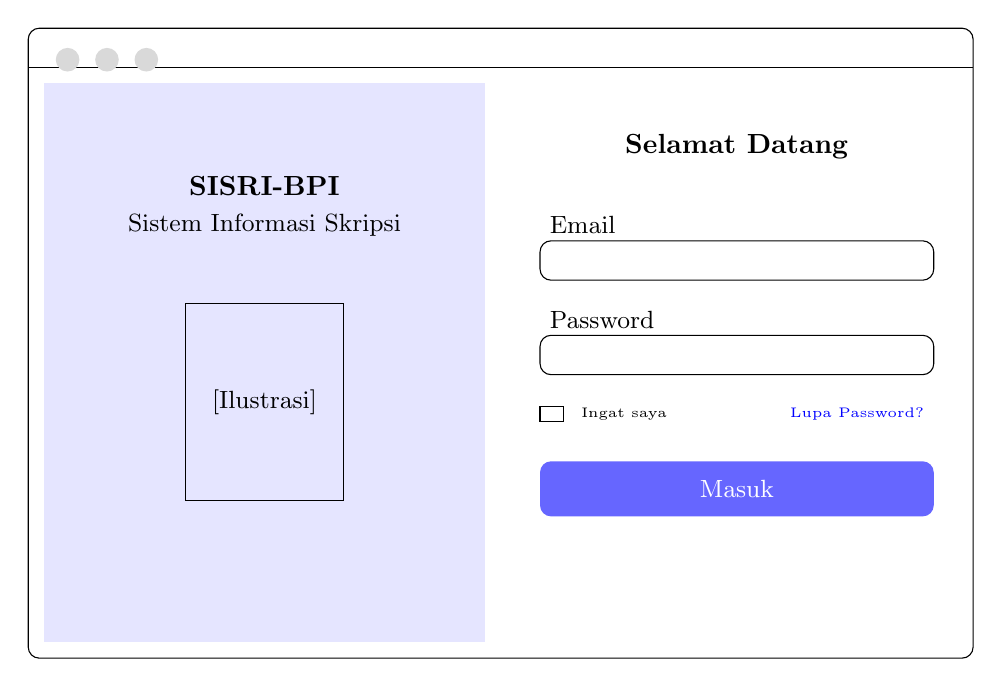
\begin{tikzpicture}
    % Browser frame
    \draw[rounded corners] (0,0) rectangle (12, 8);
    \draw (0, 7.5) -- (12, 7.5);
    \fill[gray!30] (0.5, 7.6) circle (0.15);
    \fill[gray!30] (1, 7.6) circle (0.15);
    \fill[gray!30] (1.5, 7.6) circle (0.15);
    
    % Left panel
    \fill[blue!10] (0.2, 0.2) rectangle (5.8, 7.3);
    \node at (3, 6) {\textbf{SISRI-BPI}};
    \node at (3, 5.5) {\small Sistem Informasi Skripsi};
    \draw (2, 2) rectangle (4, 4.5);
    \node at (3, 3.25) {\small [Ilustrasi]};
    
    % Right panel - Login form
    \node at (9, 6.5) {\textbf{Selamat Datang}};
    
    % Email input
    \node[anchor=west] at (6.5, 5.5) {\small Email};
    \draw[rounded corners] (6.5, 4.8) rectangle (11.5, 5.3);
    
    % Password input
    \node[anchor=west] at (6.5, 4.3) {\small Password};
    \draw[rounded corners] (6.5, 3.6) rectangle (11.5, 4.1);
    
    % Remember me & Forgot
    \draw (6.5, 3.2) rectangle (6.8, 3);
    \node[anchor=west] at (6.9, 3.1) {\tiny Ingat saya};
    \node[anchor=east] at (11.5, 3.1) {\tiny \color{blue}Lupa Password?};
    
    % Login button
    \fill[blue!60, rounded corners] (6.5, 1.8) rectangle (11.5, 2.5);
    \node[white] at (9, 2.15) {\small Masuk};
    
\end{tikzpicture}
\caption{Wireframe Halaman Login}
\label{fig:wireframe-login}
\end{figure}

\subsubsection{Halaman Dashboard Mahasiswa}
\begin{figure}[H]
\centering
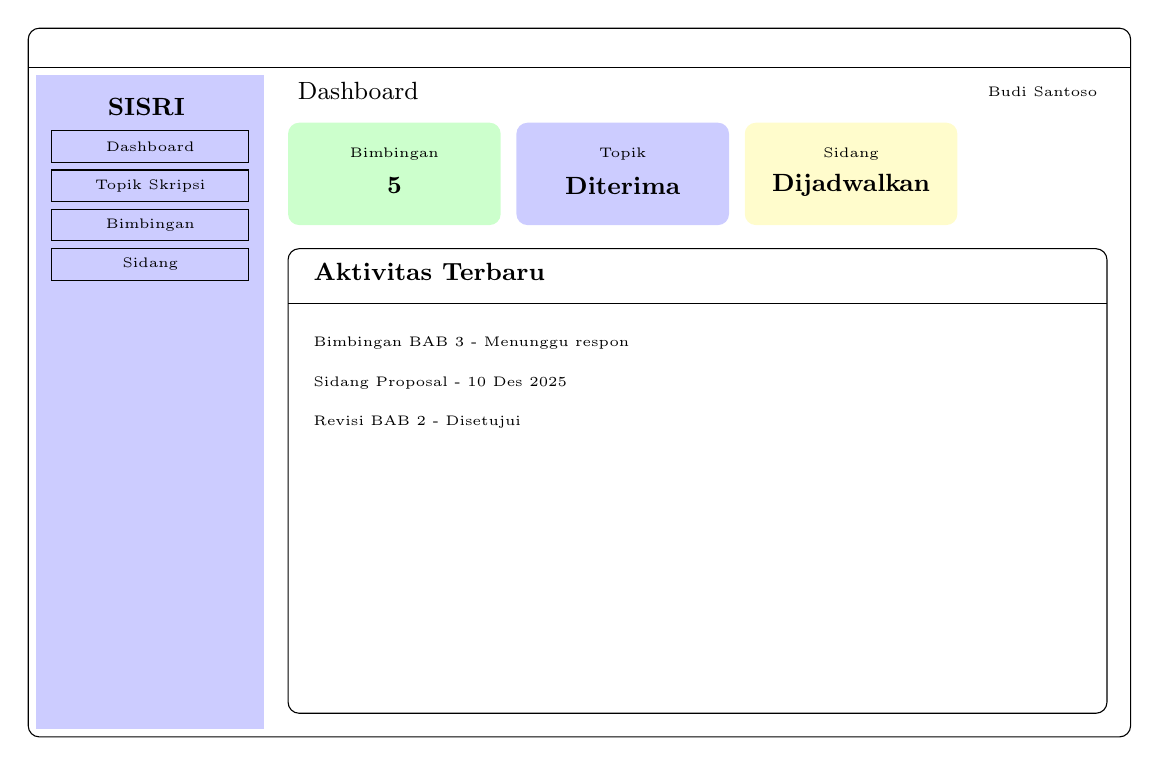
\begin{tikzpicture}
    % Browser frame
    \draw[rounded corners] (0,0) rectangle (14, 9);
    \draw (0, 8.5) -- (14, 8.5);
    
    % Sidebar
    \fill[blue!20] (0.1, 0.1) rectangle (3, 8.4);
    \node at (1.5, 8) {\small \textbf{SISRI}};
    \draw (0.3, 7.3) rectangle (2.8, 7.7);
    \node at (1.55, 7.5) {\tiny Dashboard};
    \draw (0.3, 6.8) rectangle (2.8, 7.2);
    \node at (1.55, 7) {\tiny Topik Skripsi};
    \draw (0.3, 6.3) rectangle (2.8, 6.7);
    \node at (1.55, 6.5) {\tiny Bimbingan};
    \draw (0.3, 5.8) rectangle (2.8, 6.2);
    \node at (1.55, 6) {\tiny Sidang};
    
    % Header
    \fill[white] (3.1, 8) rectangle (13.9, 8.4);
    \node[anchor=west] at (3.3, 8.2) {\small Dashboard};
    \node[anchor=east] at (13.7, 8.2) {\tiny Budi Santoso};
    
    % Stats cards
    \fill[green!20, rounded corners] (3.3, 6.5) rectangle (6, 7.8);
    \node at (4.65, 7.4) {\tiny Bimbingan};
    \node at (4.65, 7) {\small \textbf{5}};
    
    \fill[blue!20, rounded corners] (6.2, 6.5) rectangle (8.9, 7.8);
    \node at (7.55, 7.4) {\tiny Topik};
    \node at (7.55, 7) {\small \textbf{Diterima}};
    
    \fill[yellow!20, rounded corners] (9.1, 6.5) rectangle (11.8, 7.8);
    \node at (10.45, 7.4) {\tiny Sidang};
    \node at (10.45, 7) {\small \textbf{Dijadwalkan}};
    
    % Recent activity
    \draw[rounded corners] (3.3, 0.3) rectangle (13.7, 6.2);
    \node[anchor=west] at (3.5, 5.9) {\small \textbf{Aktivitas Terbaru}};
    \draw (3.3, 5.5) -- (13.7, 5.5);
    
    \node[anchor=west] at (3.5, 5) {\tiny Bimbingan BAB 3 - Menunggu respon};
    \node[anchor=west] at (3.5, 4.5) {\tiny Sidang Proposal - 10 Des 2025};
    \node[anchor=west] at (3.5, 4) {\tiny Revisi BAB 2 - Disetujui};
    
\end{tikzpicture}
\caption{Wireframe Dashboard Mahasiswa}
\label{fig:wireframe-dashboard}
\end{figure}

% ============================================
\section{Flowchart Sistem}

\subsection{Flowchart Alur Utama Skripsi}
\begin{figure}[H]
\centering
\begin{tikzpicture}[
    node distance=1cm,
    startstop/.style={ellipse, draw, minimum width=2cm, fill=green!20},
    process/.style={rectangle, draw, minimum width=3cm, minimum height=0.8cm, fill=blue!10},
    decision/.style={diamond, draw, aspect=2, fill=yellow!20},
    io/.style={trapezium, draw, trapezium left angle=70, trapezium right angle=110, minimum width=2cm, fill=orange!20},
    arrow/.style={->, thick}
]
    % Start
    \node[startstop] (start) {Mulai};
    
    % Main flow
    \node[process, below=of start] (p1) {Ajukan Topik Skripsi};
    \node[decision, below=of p1] (d1) {Disetujui?};
    \node[process, below=of d1] (p2) {Proses Bimbingan};
    \node[decision, below=of p2] (d2) {Min. 8x?};
    \node[process, below=of d2] (p3) {Daftar Sempro};
    \node[decision, below=of p3] (d3) {Lulus?};
    \node[process, right=2cm of d3] (p4) {Revisi Sempro};
    \node[process, below=of d3] (p5) {Lanjut Bimbingan};
    \node[decision, below=of p5] (d4) {Min. 8x?};
    \node[process, below=of d4] (p6) {Daftar Sidang};
    \node[decision, below=of p6] (d5) {Lulus?};
    \node[process, right=2cm of d5] (p7) {Revisi Skripsi};
    \node[startstop, below=of d5] (end) {Selesai};
    
    % Arrows
    \draw[arrow] (start) -- (p1);
    \draw[arrow] (p1) -- (d1);
    \draw[arrow] (d1) -- node[right] {Ya} (p2);
    \draw[arrow] (d1.west) -- ++(-1.5,0) |- node[near start, above] {Tidak} (p1);
    \draw[arrow] (p2) -- (d2);
    \draw[arrow] (d2) -- node[right] {Ya} (p3);
    \draw[arrow] (d2.west) -- ++(-1,0) |- node[near start, above] {Tidak} (p2);
    \draw[arrow] (p3) -- (d3);
    \draw[arrow] (d3) -- node[above] {Tidak} (p4);
    \draw[arrow] (p4) |- (p3);
    \draw[arrow] (d3) -- node[right] {Ya} (p5);
    \draw[arrow] (p5) -- (d4);
    \draw[arrow] (d4) -- node[right] {Ya} (p6);
    \draw[arrow] (d4.west) -- ++(-1,0) |- node[near start, above] {Tidak} (p5);
    \draw[arrow] (p6) -- (d5);
    \draw[arrow] (d5) -- node[above] {Tidak} (p7);
    \draw[arrow] (p7) |- (p6);
    \draw[arrow] (d5) -- node[right] {Ya} (end);
    
\end{tikzpicture}
\caption{Flowchart Alur Utama Proses Skripsi}
\label{fig:flowchart-main}
\end{figure}
